\documentclass[luatex,fontsize=8pt,paper=b5,twoside]{jlreq}%
\usepackage{amsmath,amssymb}
\usepackage{booktabs,caption,tabularx}
\usepackage{luwa-ul, KKluaverb}
\usepackage[most]{tcolorbox}
\usepackage{luatexja-ruby}
\usepackage{KKran}

% You can omit these font settings.
\makeatletter
\RequirePackage[no-math]{fontspec}
\RequirePackage[no-math,match,scale=1]{luatexja-fontspec}
\RequirePackage[hiragino-pro,deluxe,expert]{luatexja-preset}
\setmainfont{HiraMinPro-W3}[BoldFont=HiraMinPro-W6]
\setmainjfont{HiraMinPro-W3}[BoldFont=HiraMinPro-W6]
\newfontfamily{\sfhira@pre}{HiraKakuPro-W3}[BoldFont=HiraKakuPro-W6]
\newjfontfamily{\sfhiraj@pre}{HiraKakuPro-W3}[BoldFont=HiraKakuPro-W6]
\newfontfamily{\mchira@pre}{HiraMinPro-W3}[BoldFont=HiraMinPro-W6]
\newjfontfamily{\mchiraj@pre}{HiraMinPro-W3}[BoldFont=HiraMinPro-W6]
\newfontfamily{\gthira@pre}{HiraKakuPro-W3}[BoldFont=HiraKakuPro-W6,FontFace={eb}{\shapedefault}{HiraKakuStd-W8}]
\newjfontfamily{\gthiraj@pre}{HiraKakuPro-W3}[BoldFont=HiraKakuPro-W6,FontFace={eb}{\shapedefault}{HiraKakuStd-W8}]
\newfontfamily{\mghira@pre}{HiraMaruPro-W4}
\newjfontfamily{\mghiraj@pre}{HiraMaruPro-W4}
\renewcommand{\sffamily}{\sfhira@pre\sfhiraj@pre}
\renewcommand{\mcfamily}{\mchira@pre\mchiraj@pre}
\renewcommand{\gtfamily}{\gthira@pre\gthiraj@pre}
\renewcommand{\mgfamily}{\mghira@pre\mghiraj@pre}
\makeatother
%%%


\usepackage{hyperref}
\hypersetup{
  luatex, pdfencoding=auto,
  colorlinks=true,
  linkcolor=black,
  citecolor=black,
  urlcolor=DeepSkyBlue3,
  pdfborder={0 0 0},
}

\colorlet{grayLight}{white!80!black}

\NewTCBListing{SourceCode}{ m m !o !O{DeepSkyBlue3} }{%
  enhanced, colback=black!70, colframe=Snow4,
  toptitle=-1mm, bottomtitle=-1mm,
  righttitle=-1mm, lefttitle=-1mm,
  arc=.5mm,
  title={\tcbox[on line, arc=.5mm, boxsep=0pt, boxrule=0pt, top=1mm, bottom=0.8mm, left=2mm, right=2.2mm, colback=gray!80, coltext=white]{\raisebox{-0.1ex}{\vphantom{羅}\vphantom{j}#1}}},fonttitle=\gtfamily\footnotesize,boxrule=0.8pt,
  breakable,before upper={\color{white}},top=-0.5mm,bottom=-0.5mm,
  after title=\IfNoValueTF{#3}{}{{\hfill\tcbox[on line, arc=.5mm, boxsep=0pt, boxrule=0pt, top=1mm, bottom=0.8mm, left=2mm, right=2.2mm, colback=white!80!black, coltext=#4]{\raisebox{-0.1ex}{\vphantom{羅}\vphantom{j}#3}}}},
  listing only,
  listing options={
    language={#2},
    basicstyle=\ttfamily,
    keywordstyle=\ttfamily\color{white},
    stringstyle=\itshape\color{white},
    commentstyle=\small\gtfamily\color{DeepSkyBlue2},
    showspaces=false,showtabs=false,
    breaklines=true,breakindent=0pt,
    showstringspaces=false,
    columns=fullflexible,
    tabsize=2,
    numbers=left,numbersep=1.5pt,
    numberstyle=\scriptsize\gtfamily\color{gray},
  }
}

\NewTColorBox{OutPut}{ m !o !O{DeepSkyBlue3} }{%
  enhanced, colframe=Snow4,
  toptitle=-1mm, bottomtitle=-1mm,
  righttitle=-1mm, lefttitle=-1mm,
  arc=.5mm, colback=white,
  title={\tcbox[on line, arc=.5mm, boxsep=0pt, boxrule=0pt, top=1mm, bottom=0.8mm, left=2mm, right=2.2mm, colback=gray!40, coltext=DeepSkyBlue3]{\raisebox{-0.1ex}{\vphantom{羅}\vphantom{j}#1}}},fonttitle=\gtfamily\footnotesize,boxrule=0.8pt,
  breakable,top=-0.5mm,bottom=-0.5mm,
  after title=\IfNoValueTF{#2}{}{{\hfill\tcbox[on line, arc=.5mm, boxsep=0pt, boxrule=0pt, top=1mm, bottom=0.8mm, left=2mm, right=2.2mm, colback=white!80!black, coltext=#3]{\raisebox{-0.1ex}{\vphantom{羅}\vphantom{j}#2}}}}, bottom=2mm, top=2mm,
}

\title{\texttt{KKran} Package Documentation}
\author{Kosei Kawaguchi a.k.a. KKTeX}
\date{Version 1.2.1 (2026/09/30)}

\begin{document}
\begin{titlepage}
  \maketitle
\end{titlepage}
\newpage
\tableofcontents
\newpage


\section{まず使ってみる / Quick start}
\texttt{KKran}は試験用の解答欄を組み立てるLuaLaTeX専用のパッケージです。
番号・解答欄・改行を順に指定し、一つの\KKverb|\KKran|でまとめます。
横組みと縦組みに対応します。マークシートは横組みで使うことを推奨します。

\textbf{English.} Build answer sheets from numbered boxes, rows and grids.
Compile with LuaLaTeX. KKsymbols 2.3.1 or later is required.

\begin{SourceCode}{Input}{TeX}[最小の文書 / Minimal document]
\documentclass{jlreq}
\usepackage[kaitouhyouji=0]{KKran}
\begin{document}
\KKran{%
  \大問番号{4}
  \小問番号{2}\小問欄{5}{2}\GoDown{2}
  \小問番号{2}\小問欄{5}{2}
}
\end{document}
\end{SourceCode}
\begin{OutPut}{Output}
\KKran{\大問番号{4}\小問番号{2}\小問欄{5}{2}\GoDown{2}\小問番号{2}\小問欄{5}{2}}
\end{OutPut}

\paragraph{幅と高さの読み方}
\KKverb|\小問欄{5}{2}|は「幅5マス、高さ2マス」です。
1マスの幅は\KKverb|unit|で指定し、既定値は\KKverb|2\zw|です。
\KKverb|\GoDown{2}|は2マス下へ移動し、大問番号の右端から次の段を始めます。


\subsection{目的から選ぶ}
{\small
\noindent\begin{tabularx}{\linewidth}{@{}lX@{}}
\toprule
作りたいもの & コマンド\\\midrule
番号付きの解答欄 & \KKverb|\小問番号{高さ}\小問欄{幅}{高さ}|\\
同じ小問の複数の欄 & 途中の欄は\KKverb|\小問中欄|、最後は\KKverb|\小問欄|\\
次の段 & \KKverb|\GoDown{移動量}|\\
大問番号 & \KKverb|\大問番号[幅]{高さ}|\\
マス目付きの記述欄 & \KKverb|\小問マス目[文字数下限]{文字数上限}|\\
模範解答 & \KKverb|\KaitouInput{解答}|\\
マークシート & \KKverb|\MarkArrayMake|で配列を作り、\KKverb|\マークシート|で出力\\
\bottomrule
\end{tabularx}}\par\medskip

\subsection{読み込みと解答表示}
\texttt{KKran.sty}をTeXの検索対象ディレクトリへ配置します。
\texttt{KKsymbols} 2.3.1以降も必要です。設定一覧は\ref{sec:ran-options}節を参照してください。

\begin{SourceCode}{Input}{TeX}[配布用と解答用を切り替える]
\usepackage[kaitouhyouji=0]{KKran} % 生徒用：模範解答を隠す
% \usepackage[kaitouhyouji=1]{KKran} % 解答用（既定値）
\end{SourceCode}
\textbf{注意：既定では模範解答が表示されます。} 生徒用は\KKverb|kaitouhyouji=0|を指定してください。
別の描画命令で明示的に色を指定した部分は隠れない場合があります。模範解答の節も確認してください。

\section{使い方}
\subsection{\KKverb|\KKran|}
解答欄を構成するコマンドを、\KKverb|\KKran|の必須引数に順に並べます。前の省略可能引数は外枠の線幅、後ろは番号の形式です。

\begin{SourceCode}{Input}{TeX}
  \KKran[解答欄の外枠を囲む線の太さ]{引数}[ナンバリングのオプション]
\end{SourceCode}

\noindent という構文です。

ナンバリングのオプションとは、番号をどの形式で進めるかを指定するもので、

\begin{SourceCode}{Input}{TeX}
  \KKran[解答欄の外枠を囲む線の太さ]{引数}[%
    daimon=いろは, shoumon=一
  ]
\end{SourceCode}

\noindent のような書き方をします。それぞれ何も指定しない場合は、アラビア数字でカウントされますが、そうでないカウント方法を取りたい場合、以下の選択肢から選ぶことになります。

\begin{description}
  \item[\KKverb|daimon|] a, A, あ, ア, いろは, イロハ, 一, ロ小, ロ大を取れます。それぞれ、abc\dots, ABC\dots, あいう\dots, アイウ\dots, いろは\dots, イロハ\dots, 一二三\dots, \Rrnum*{1} \ \Rrnum*{2} \ \Rrnum*{3}\dots, \Rrnum{1} \ \Rrnum{2} \ \Rrnum{3}\dots というカウント形式です。
  \item[\KKverb|shoumon|] 上に同じです。
\end{description}

\subsection{ローマ数字の大小文字と小文字用の基準}
\KKverb|\Rrnum| は、スターなしで大文字、スター付きで小文字のローマ数字を
出力します。

\begin{SourceCode}{Input}{TeX}
  \Rrnum{8}   % VIII
  \Rrnum*{8}  % viii
\end{SourceCode}

小文字ローマ数字は \texttt{i}、\texttt{v}、\texttt{x} などで実際の高さが異なります。
そのため、独自に小文字ローマ数字をマークシートの囲みへ入れる場合は、囲みを
出力する前に \texttt{KKsymbols} の \KKverb|\kksref| で共通の phantom 基準を
設定してください。効果はグループ内に限定するのが安全です。

\begin{SourceCode}{Input}{TeX}
  \MarkArrayMake{ローマ小}{%
    |\Rrnum*{1}|\Rrnum*{2}|\Rrnum*{3}|\Rrnum*{4}|\Rrnum*{5}|}
  {\kksref{\Rrnum*{6}}% vi を共通の高さ・深さの基準にする
    \マークシート{5}{\ローマ小マーク配列}}
\end{SourceCode}

\KKverb|daimon=ロ小| および \KKverb|shoumon=ロ小| は、同じ
\KKverb|\kksref{\Rrnum*{6}}| を番号スタイルへ適用する前に内部で設定します。
独自の番号内容や独自の囲みを使う場合には、上の例のように利用者側で先に
設定してください。大文字ローマ数字には通常この前処理は不要です。

\subsection{小問}
番号は\verb|\小問番号|、解答欄は\verb|\小問欄|で作ります。同じ小問内で欄を分ける場合は、途中の欄に\verb|\小問中欄|を使います。

\begin{SourceCode}{Input}{TeX}
  % 構文
  \小問番号[横幅]{縦幅}[番号]
  % デフォルト
  % 横幅：.5
  % 番号：アラビア数字（\kakkoに入っている）

  % 使用例
  \KKran{%
    \小問番号[1]{2}\小問番号{2}[A]\小問番号{2}[B]\小問番号[1]{2}\小問番号[1]{2}
  }
\end{SourceCode}

\noindent が基本構文です。

出力は

\begin{OutPut}{Output}
  \KKran{%
    \小問番号[1]{2}\小問番号{2}[A]\小問番号{2}[B]\小問番号[1]{2}\小問番号[1]{2}
  }
\end{OutPut}

\noindent のようになります。

第３引数を指定しない場合、小問番号のカウンタは自動で進みますが、ここを手動で書いた場合はカウンタが進みません。
カウンタを強制的にある値にしたい場合には、\verb|\SetShoumon{99}|のように変更できるようにしてあります。

また、当然ながら大問が変わると値はリセットされます（大問の分け方は後述）。

ここに、\verb|\小問欄|および\verb|小問中欄|を組み合わせます。

\begin{SourceCode}{Input}{TeX}
  % 構文
  \小問欄{横幅}{縦幅}[欄内記入]
  \小問中欄{横幅}{縦幅}[欄内記入]
  % デフォルト
  % 欄内記入：空集合

  % 使用例
  \KKran{%
    \小問番号{2}\小問中欄{3}{2}\小問中欄{3}{2}\小問欄{4}{2}[south east={$\mathrm{mm}$}, west={$x=$}]\小問番号{2}\小問欄{4}{2}
  }
\end{SourceCode}

\begin{OutPut}{Output}
  \KKran{%
    \小問番号{2}\小問中欄{3}{2}\小問中欄{3}{2}\小問欄{4}{2}[south east={$\mathrm{mm}$}, west={$x=$}]\小問番号{2}\小問欄{4}{2}
  }
\end{OutPut}

基本的には\verb|\小問欄|を使いますが、同一の小問内で複数解答欄を用意する時などは、最後の欄以外を\verb|\小問中欄|にしても良いでしょう。

欄内の配置位置は、\KKverb|center|、\KKverb|east|、\KKverb|west|、\KKverb|north east|、\KKverb|north west|、\KKverb|south east|、\KKverb|south west|から選びます。
指定した位置を基準として内容を配置します。TikZのnodeと同じ指定方法です。

引数には何を挿入してもよく、図表も挿入可能です。

\begin{SourceCode}{Input}{TeX}
  \KKran{
    \小問番号{6}\小問欄{8}{6}[center={%
      \begin{tabular}{|l|c|r|}
      \hline
      列1 & 列2 & 列3 \\ \hline
      データA & 100 & 5.5 \\ \hline
      データB & 200 & 9.8 \\ \hline
      データC & 300 & 12.3 \\ \hline
      \end{tabular}
    }]
    \小問番号{6}\小問欄{9}{6}[center={%
      \begin{tikzpicture}
        \draw[->] (0, -.3) -- (0, 2.5) node[above] {$y$};
        \draw[->] (-2, 0) -- (2, 0) node[right] {$x$};
        \filldraw (0, 0) circle (.5pt) node[below left] {$\mathrm{O}$};
        \draw[domain=-1.5:1.5, samples=100, thick] plot (\x, {\x*\x});
      \end{tikzpicture}
    }]
  }
\end{SourceCode}

\begin{OutPut}{Output}
  \KKran{
    \小問番号{6}\小問欄{8}{6}[center={%
      \begin{tabular}{|l|c|r|}
      \hline
      列1 & 列2 & 列3 \\ \hline
      データA & 100 & 5.5 \\ \hline
      データB & 200 & 9.8 \\ \hline
      データC & 300 & 12.3 \\ \hline
      \end{tabular}
    }]
    \小問番号{6}\小問欄{9}{6}[center={%
      \begin{tikzpicture}
        \draw[->] (0, -.3) -- (0, 2.5) node[above] {$y$};
        \draw[->] (-2, 0) -- (2, 0) node[right] {$x$};
        \filldraw (0, 0) circle (.5pt) node[below left] {$\mathrm{O}$};
        \draw[domain=-1.5:1.5, samples=100, thick] plot (\x, {\x*\x});
      \end{tikzpicture}
    }]
  }
\end{OutPut}

\subsection{模範解答入力}
模範解答を入力する場合、その部分を\verb|\KaitouInput{引数}|によって入力しておくと、パッケージオプションである\texttt{kaitouhyouji}が1の時だけ表示されるようになります。ただし、この効果は\verb|\color|コマンドによる色の変更が可能な範囲に限ります。

tikzの描画も当然解答として入力可能ですが、

\begin{SourceCode}{Input}{TeX}
  \KKran{
    \小問番号{6}\小問欄{9}{6}[center={\KaitouInput{%
      \begin{tikzpicture}
        \draw[->] (0, -.3) -- (0, 2.5) node[above] {$y$};
        \draw[->] (-2, 0) -- (2, 0) node[right] {$x$};
        \filldraw (0, 0) circle (.5pt) node[below left] {$\mathrm{O}$};
        \draw[domain=-1.5:1.5, samples=100, thick, blue] plot (\x, {\x*\x}); % ここ！
      \end{tikzpicture}
    }}]
  }
\end{SourceCode}

\begin{OutPut}{Output}
    \KKran{
    \小問番号{6}\小問欄{9}{6}[center={\KaitouInput{%
      \begin{tikzpicture}
        \draw[->] (0, -.3) -- (0, 2.5) node[above] {$y$};
        \draw[->] (-2, 0) -- (2, 0) node[right] {$x$};
        \filldraw (0, 0) circle (.5pt) node[below left] {$\mathrm{O}$};
        \draw[domain=-1.5:1.5, samples=100, thick, blue] plot (\x, {\x*\x}); % ここ！
      \end{tikzpicture}
    }}]
  }
\end{OutPut}

明示的に色を指定した部分には、\verb|\KaitouInput|による表示切り替えが適用されません。

\section{大問ごとの組み方}
\verb|\大問番号|で大問番号を置き、その右に解答欄を並べます。次の段へ進むときは\verb|\GoDown|で下への移動量を指定します。

\begin{SourceCode}{Input}{TeX}
  % 構文
  \大問番号[横幅]{縦幅}[番号]
  % デフォルト
  % 横幅：.5
  % 番号：アラビア数字（\kakkoに入っている）

  \GoDown{下に降りたいマス目数}

  % 使用例
  \KKran[3pt]{%
    \大問番号[1]{9}
    \小問番号{2}\小問欄{2}{2}\小問番号{2}\小問欄{4}{2}\GoDown{2}
    \小問番号{4}\小問欄{8}{4}\GoDown{4}
    \小問番号{3}\小問欄{3}{3}\小問番号{3}\小問欄{2}{3}
  }[shoumon=いろは,daimon=ア]
\end{SourceCode}

\begin{OutPut}{Output}
  \KKran[3pt]{%
    \大問番号[1]{9}
    \小問番号{2}\小問欄{2}{2}\小問番号{2}\小問欄{4}{2}\GoDown{2}
    \小問番号{4}\小問欄{8}{4}\GoDown{4}
    \小問番号{3}\小問欄{3}{3}\小問番号{3}\小問欄{2}{3}
  }[shoumon=いろは,daimon=ア]
\end{OutPut}

大問番号をある値にしたいという場合、\verb|\SetDaimon{99}|のように指定します。

\section{記述解答欄}
記述問題専用の解答欄として、マス目ありのもの、なしのものの２種類の解答欄を用意しています。

注意点として、\verb|\linewidth|を上回る横幅を解答欄が占めるような組み方をしてはならないというものがあります。エラーにはなりませんが、大問と大問との間隔が余計に１行分大きくなってしまいます。

\begin{SourceCode}{Input}{TeX}
  % 構文
  \小問マス目[文字数下限]{文字数上限}[欄内記入]
  \小問記述{文字数上限}[欄内記入]
  % デフォルト
  % 文字数下限：文字数上限と同じ値
  % 欄内記入：空集合

  % 使用例
  \KKran[3pt]{%
    \大問番号[1]{7}
    \小問番号{1}\小問マス目[4]{6}\GoDown{1}
    \小問番号{2}\小問記述{40}\GoDown{2}
    \小問番号{4}\小問マス目[50]{75}
  }
\end{SourceCode}

\begin{OutPut}{Output}
  \noindent\resizebox{\linewidth}{!}{%
  \KKran[3pt]{%
    \大問番号[1]{7}
    \小問番号{1}\小問マス目[4]{6}\GoDown{1}
    \小問番号{2}\小問記述{40}\GoDown{2}
    \小問番号{4}\小問マス目[50]{75}
  }}
\end{OutPut}

また、ここに模範解答を入力する際は半角英数字や約物を全角１マスに適切に拡大縮小するため、必要に応じて\verb|\全角幅固定|というコマンドを使用します。

\begin{SourceCode}{Input}{TeX}
  % 使用例
  \KKran[3pt]{%
    \大問番号[1]{3}
    \小問番号{1}\小問マス目[4]{6}[\KaitouInput{\全角幅固定{12}\全角幅固定{3}番目\全角幅固定{。}}]\GoDown{1}
    \小問番号{2}\小問マス目{40}[\KaitouInput{\全角幅固定{「}日本に\全角幅固定{Ma}\全角幅固定{tt}\全角幅固定{he}\全角幅固定{w\phantom{w}}＝\全角幅固定{Pe}\全角幅固定{rr}\全角幅固定{y\phantom{y}}提督が来たから。\全角幅固定{」}という話であります。}]
  }
\end{SourceCode}

\begin{OutPut}{Output}
  \noindent\resizebox{\linewidth}{!}{%
  \KKran[3pt]{%
    \大問番号[1]{3}
    \小問番号{1}\小問マス目[4]{6}[\KaitouInput{\全角幅固定{12}\全角幅固定{3}番目\全角幅固定{。}}]\GoDown{1}
    \小問番号{2}\小問マス目{40}[\KaitouInput{\全角幅固定{「}日本に\全角幅固定{Ma}\全角幅固定{tt}\全角幅固定{he}\全角幅固定{w\phantom{w}}＝\全角幅固定{Pe}\全角幅固定{rr}\全角幅固定{y\phantom{y}}提督が来たから。\全角幅固定{」}という話であります。}]
  }}
\end{OutPut}

\section{マークシート}
最初に\verb|\MarkArrayMake|で選択肢の配列を作り、\verb|\マークシート|で配置します。
マークシートは横組みでの使用を想定しています。
縦組みの文書では、\texttt{lltjext}などで部分的に横組みにして配置してください。

\begin{SourceCode}{Input}{TeX}
  % 構文
  \MarkArrayMake{配列名}{|要素1|要素2|...|要素n|}
  \マークシート{配置幅}{配列格納}[正解番号]

  % 使用例
  \MarkArrayMake{テストA}{|$\pm$|0|1|2|3|}
  \MarkArrayMake{テストB}{|ア|イ|ウ|エ|オ|}
  \KKran[3pt]{%
    \大問番号[1]{8}
    \小問番号{1}\小問欄{6}{1}[center=\マークシート{5}{\テストAマーク配列}[4]]\GoDown{1}
    \小問番号{1}\小問欄{6}{1}[center=\マークシート{5}{\テストAマーク配列}[1]]\GoDown{1}
    \小問番号{1}\小問欄{6}{1}[center=\マークシート{5}{\テストAマーク配列}[4]]\GoDown{1}
    \小問番号{1}\小問欄{6}{1}[center=\マークシート{5}{\テストBマーク配列}[3]]\GoDown{1}
    \小問番号{1}\小問欄{6}{1}[center=\マークシート{5}{\テストBマーク配列}[2]]\GoDown{1}
    \小問番号{1}\小問欄{6}{1}[center=\マークシート{5}{\テストBマーク配列}[3]]\GoDown{1}
    \小問番号{1}\小問欄{6}{1}[center=\マークシート{5}{\テストBマーク配列}[4]]\GoDown{1}
    \小問番号{1}\小問欄{6}{1}[center=\マークシート{5}{\テストBマーク配列}[3]]\GoDown{1}
  }[shoumon=一,daimon=ア]
\end{SourceCode}

\begin{OutPut}{Output}
  \MarkArrayMake{テストA}{|$\pm$|0|1|2|3|}
  \MarkArrayMake{テストB}{|ア|イ|ウ|エ|オ|}
  \KKran[3pt]{%
    \大問番号[1]{8}
    \小問番号{1}\小問欄{6}{1}[center=\マークシート{5}{\テストAマーク配列}[4]]\GoDown{1}
    \小問番号{1}\小問欄{6}{1}[center=\マークシート{5}{\テストAマーク配列}[1]]\GoDown{1}
    \小問番号{1}\小問欄{6}{1}[center=\マークシート{5}{\テストAマーク配列}[4]]\GoDown{1}
    \小問番号{1}\小問欄{6}{1}[center=\マークシート{5}{\テストBマーク配列}[3]]\GoDown{1}
    \小問番号{1}\小問欄{6}{1}[center=\マークシート{5}{\テストBマーク配列}[2]]\GoDown{1}
    \小問番号{1}\小問欄{6}{1}[center=\マークシート{5}{\テストBマーク配列}[3]]\GoDown{1}
    \小問番号{1}\小問欄{6}{1}[center=\マークシート{5}{\テストBマーク配列}[4]]\GoDown{1}
    \小問番号{1}\小問欄{6}{1}[center=\マークシート{5}{\テストBマーク配列}[3]]\GoDown{1}
  }[shoumon=一,daimon=ア]
\end{OutPut}

\verb|\マークシート{配置幅}{配列格納}[正解番号]|の第３引数で指定した番号を$n \in \mathbb{N}$として、作成した配列の$n$番目が黒く塗られる仕様となっており、模範解答の入力はこれで行います。\verb|kaitouhyouji=0|の時は塗られず、\verb|kaitouhyouji=1|のときにのみ黒く塗った部分が表示されます。

配列要素に小文字ローマ数字を使う場合は、\KKverb|\マークシート| を出力する
前に、グループの先頭で \KKverb|\kksref{\Rrnum*{6}}| を指定してください。
これにより各要素へ共通の \KKverb|\vphantom| 相当の基準が入り、文字ごとの高さの
違いが囲みの大きさや位置へ反映されるのを防ぎます。具体例は
「ローマ数字の大小文字と小文字用の基準」を参照してください。

\section{設定一覧}\label{sec:ran-options}
\verb|\usepackage[オプション]{KKran}|により読み込みます。

以下のオプションを\KKverb|\usepackage[...]{KKran}|で指定します。
内部では\texttt{calc, tikz, xcolor, KKsymbols, kvoptions, pgfkeys, luacode, etoolbox}を読み込みます。

\begin{description}
  \item[\KKverb|kaitouhyouji|] 解答欄上に模範解答を出力するか否かを指定します。"0"なら出力せず、"1"なら出力します。既定値は１です。
  \item[\KKverb|kaitoucolor|] 模範解答の文字の色を指定します。既定値はredです。
  \item[\KKverb|gridmax|] マス目を出力するコマンドである\verb|\小問マス目| において、１行当たりの最大マス目数を指定します。既定値は20です。
  \item[\KKverb|nongridmax|] 記述解答欄を出力するコマンドである\verb|\小問記述| において、１行当たりの最大マス目数を指定します。ただし、このコマンドではマス目は可視化されません。既定値は20です。
  \item[\KKverb|unit|] 本パッケージでは「マス目単位で」各解答欄の位置を制御します。その際の１マスの幅を指定するのがこのオプションです。既定値は\verb|2\zw|です。
  \item[\KKverb|wakuwidth|] 解答欄の枠線の太さを指定します。既定値は\verb|.7pt|です。
  \item[\KKverb|tensenwakuwidth|] 欄の一部に使われている点線部分の太さを指定します。既定値は\verb|.4pt|です。
  \item[\KKverb|tensenon|] 欄の一部に使われている点線部分のdash-patternを決めるためのもので、線の最小単位の長さを指定できます。既定値は\verb|1pt|です。
  \item[\KKverb|tensenoff|] 欄の一部に使われている点線部分のdash-patternを決めるためのもので、最小単位の配置間隔を指定できます。既定値は\verb|1pt|です。
  \item[\KKverb|clsadjust|] jlreqクラス以外を指定する場合は、\verb|clsadjust=1|を指定します。一部クラスにおいて\verb|\小問マス目|に解答を入力した際、字間の調整が適切になされない事例があるためです。この値の既定値は0になっています。このオプションは内部的に、\verb|clsadjust=1|のとき
  \KKcodeS+
    \RequirePackage[scale=1]{luatexja-fontspec}
    \RequirePackage[deluxe,expert]{luatexja-preset}
  \KKcodeE
  \noindent を読み込むという処理をしています。したがって、より詳細にこれらのオプションを設定したい場合には\verb|clsadjust=0|とし、適宜設定をしてください。
  \item[\KKverb|fontdaimonbangou| / \KKverb|fontshoumonbangou|] 大問番号／小問番号のフォントを\verb|\gtfamily|や\verb|\small|のような形式で指定します。既定値は\verb|\relax|（つまり指定なし）です。
  \item[\KKverb|styledaimonbangou| / \KKverb|styleshoumonbangou|] 大問番号／小問番号のスタイルを指定します。指定するのは「制御綴名」です。例えば``\verb|\maru{引数}|''（\verb|KKsymbols|パッケージが提供）を使用して小問番号を丸数字にしたいという場合、\verb|styleshoumonbangou=maru|とします。既定値は\verb|kakko|となっています。特に括弧や丸などをつけたくない場合、\verb|全角幅固定|と指定するのが推奨されます。
\end{description}


\clearpage
\appendix
\section{解答用紙の全体サンプル}
\begin{SourceCode}{Input}{TeX}
  \documentclass[paper=a4]{jlreq}

  \usepackage[
    kaitouhyouji=1,
    gridmax=20,
    kaitoucolor=red,
    fontdaimonbangou=\gtfamily,
    styledaimonbangou=全角幅固定
  ]{KKran}

  \begin{document}
  \KKran{%
    \大問番号{9}
    \小問番号{2}\小問欄{2}{2}[center=\KaitouInput{ア}]\小問番号{2}\小問中欄{5}{2}[west=人物：,center=\KaitouInput{松尾},east=芭蕉]\小問欄{6}{2}[west=作品：,center=\KaitouInput{奥の細道}]\GoDown{2}
    \小問番号{2}\小問欄{4}{2}[center=\KaitouInput{つわもの}]\小問番号{2}\小問欄{2}{2}[center=\KaitouInput{ウ}]\小問番号{2}\小問欄{2}{2}[center=\KaitouInput{エ}]
    \小問番号{2}\小問欄{4}{2}[center=\KaitouInput{片雲の風}]
    \小問番号{2}\小問欄{5}{2}[center=\KaitouInput{春夜宴桃李園序}]\GoDown{2}
    \小問番号{4}\小問マス目[45]{65}[\KaitouInput{李白の著名な詩を元にした\全角幅固定{「}月日は百代の過客\全角幅固定{」}という表現を引いて旅に主題を仄めかしつつ\全角幅固定{、}滑らかにに自身の紀行文に主眼を移す役割\全角幅固定{。}}]\GoDown{4}
    \小問番号{1}\小問マス目{7}[\KaitouInput{道祖神の招き}]
  }[shoumon=a,daimon=ア]
  \bigskip

  \KKran{%
    \大問番号{10}\小問番号{2}\小問欄{3}{2}[center=\KaitouInput{144}]\小問番号{2}\小問欄{4}{2}[south east={$\mathrm{mm}$},center=\KaitouInput{$3.0$}, west={$x=$}]\GoDown{2}
    \小問番号{8}\小問欄{9}{8}[center={\KaitouInput{%
      \begin{tikzpicture}
        \draw[domain=-1.5:1.5, samples=100, thick] plot (\x, {\x*\x});
        \draw[->,, black] (0, -.3) -- (0, 2.5) node[above] {$y$};
        \draw[->,, black] (-2, 0) -- (2, 0) node[right] {$x$};
        \filldraw[black] (0, 0) circle (.5pt) node[below left] {$\mathrm{O}$};
      \end{tikzpicture}}}]
  }[shoumon=一,daimon=ア]
  \bigskip

  \MarkArrayMake{テストA}{|$\pm$|0|1|2|3|}
  \MarkArrayMake{テストB}{|ア|イ|ウ|エ|オ|}
  \KKran{%
    \大問番号{8}
    \小問番号{1}\小問欄{6}{1}[center=\マークシート{5}{\テストAマーク配列}[4]]\GoDown{1}
    \小問番号{1}\小問欄{6}{1}[center=\マークシート{5}{\テストAマーク配列}[1]]\GoDown{1}
    \小問番号{1}\小問欄{6}{1}[center=\マークシート{5}{\テストAマーク配列}[4]]\GoDown{1}
    \小問番号{1}\小問欄{6}{1}[center=\マークシート{5}{\テストBマーク配列}[3]]\GoDown{1}
    \小問番号{1}\小問欄{6}{1}[center=\マークシート{5}{\テストBマーク配列}[2]]\GoDown{1}
    \小問番号{1}\小問欄{6}{1}[center=\マークシート{5}{\テストBマーク配列}[3]]\GoDown{1}
    \小問番号{1}\小問欄{6}{1}[center=\マークシート{5}{\テストBマーク配列}[4]]\GoDown{1}
    \小問番号{1}\小問欄{6}{1}[center=\マークシート{5}{\テストBマーク配列}[3]]\GoDown{1}
  }[shoumon=ロ小,daimon=ア]

  \end{document}
\end{SourceCode}

\begin{OutPut}{Output}
  \begin{center}
    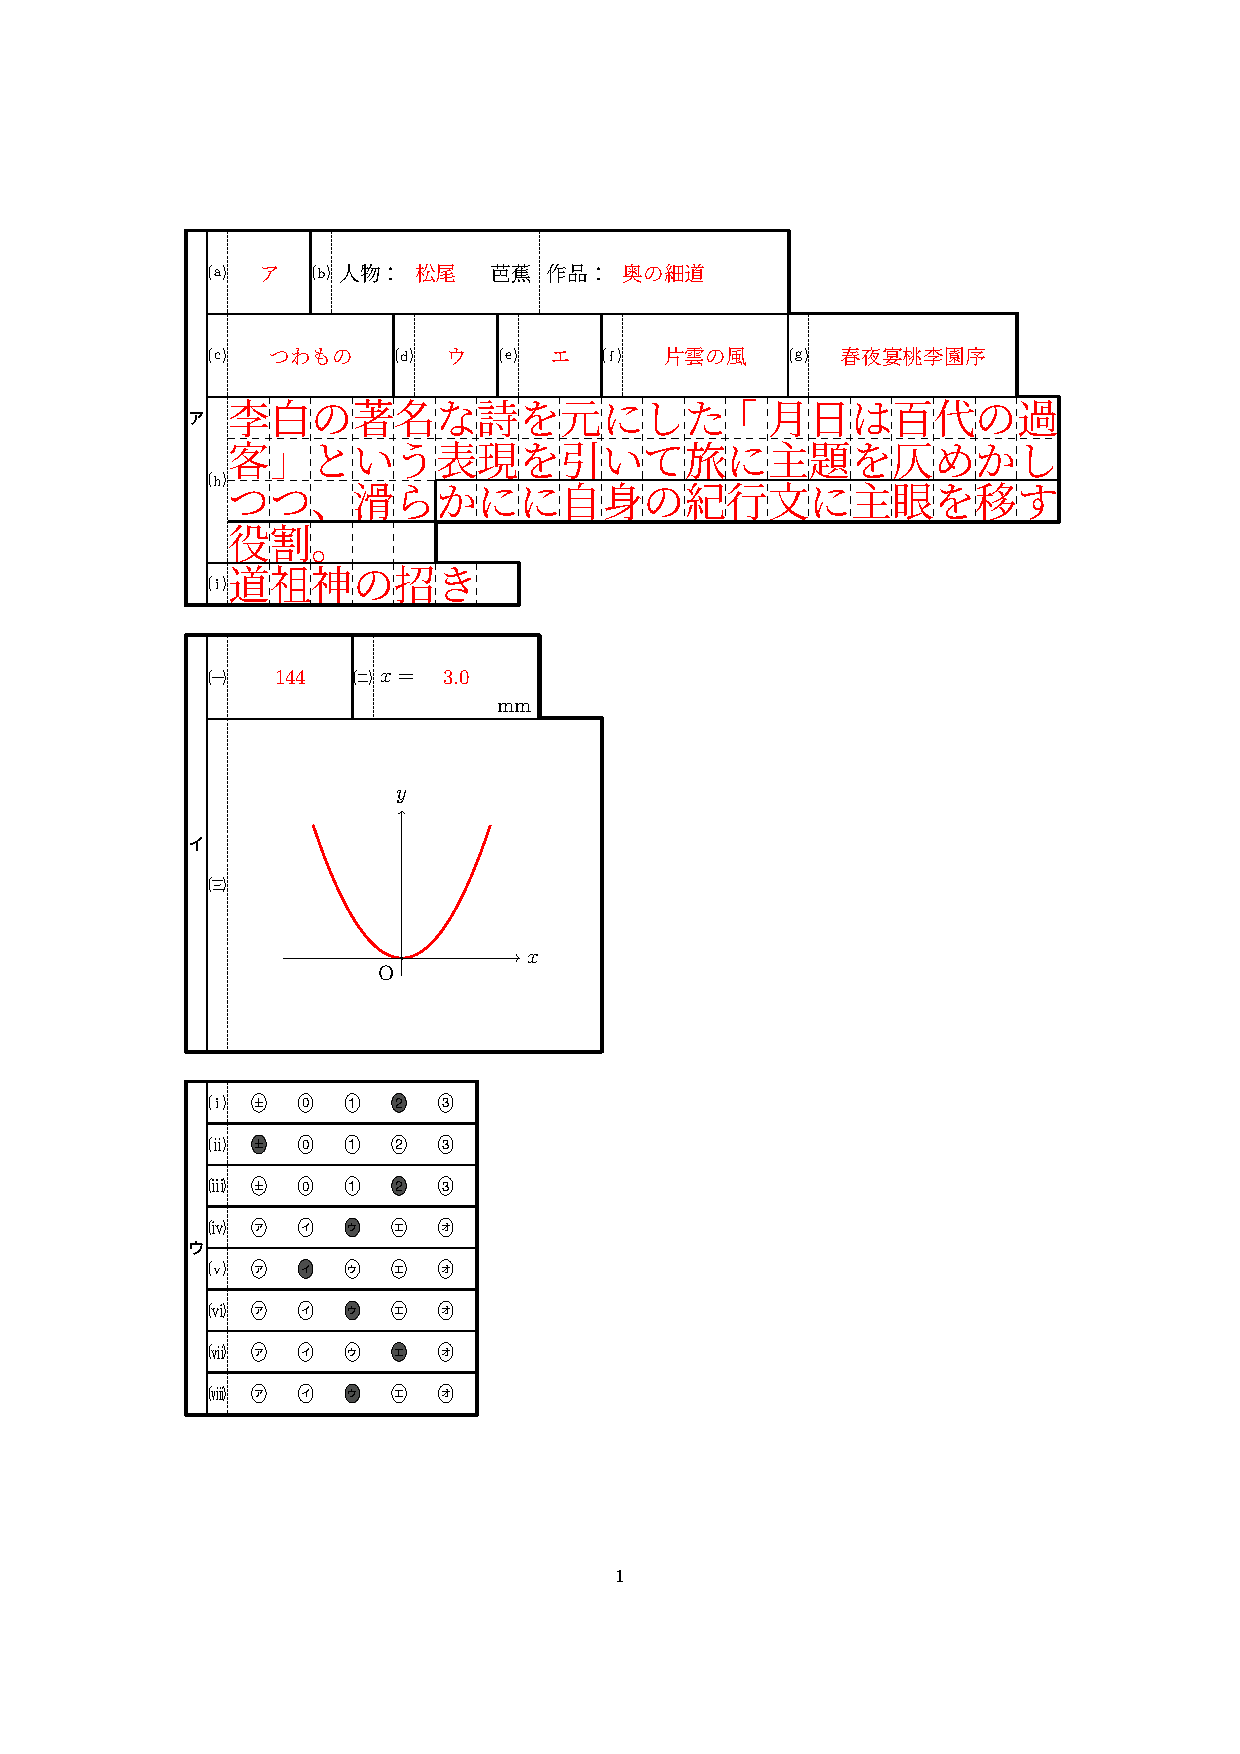
\includegraphics[width=.7\columnwidth]{kkran-sample.pdf}
  \end{center}
\end{OutPut}


\section{Version History}
\begin{itemize}
  \item \textbf{v1.0.0 (2025/11/23)} --- Initial public release.
  \item \textbf{v1.1.0 (2025/12/23)} --- Changed internal behavior in order to follow KKsymbols v2.0.0
  \item \textbf{v1.1.2 (2026/01/02)} --- Added license file and improved README file. In addition, the manual has been updated to reflect bug fixes introduced in luatexja version 20260107.0.
  \item \textbf{v1.1.4 (2026/02/15)} --- I changed the following points:
  \begin{itemize}
    \item Fixed a bug where the left border of \verb|\小問欄|, \verb|\小問中欄|, \verb|\小問マス目|, and \verb|\小問記述| produce unwanted thin line.
    \item Add some package options in order to set font and style of ``大問番号'' and ``小問番号''.
    \item Add a new command \verb|\全角幅固定| to input ``半角英数字'' to the optional argument of \verb|\小問マス目|.
    \item Changed some dafault values of package options.
  \end{itemize}
  \item \textbf{v1.1.5 (2026/02/17)} --- Fixed a bug where unwanted ``\KKverb|*|'' is output when \KKverb|styledaimonbangou| or \KKverb|styleshoumonbangou| is set to \KKverb|全角幅固定| and the optional argument of \KKverb|\KKran| is set as \KKverb|[shoumon=a]| or \KKverb|[daimon=a]|.
  \item \textbf{v1.1.6 (2026/02/20)} --- Improved the output of the dashed lines of \KKverb|\小問マス目|.
  \item \textbf{v1.2.0 (2026/08/20)} --- Loaded KKsymbols explicitly with \KKverb|autolowercase=1|, changed \KKverb|\Rrnum| so its starred form produces lowercase Roman numerals, and applied \KKverb|\kksref| before built-in lowercase Roman numbering.
  \item \textbf{v1.2.1 (2026/09/30)} --- Preserve explicitly selected KKsymbols options, including \KKverb|autolowercase=0|, without an option clash. Require KKsymbols 2.3.1 for consistent Roman-numeral classification.
\end{itemize}


\end{document}
